\documentclass[a4paper]{article}
\usepackage[german]{babel}

\usepackage{ucs}
\usepackage[utf8x]{inputenc}

\usepackage{graphicx}
\usepackage{subfigure} % Bilder platzieren(z.B. nebeneinander)
\graphicspath{{.}}

\newcommand{\HRule}{\rule{\linewidth}{0.25mm}}


\begin{document}
\begin{titlepage}
  \begin{center}
    
\includegraphics[width=0.25\textwidth]{myselogo}\\[1cm]
    \textsc{\LARGE Systems Engineering Group\\[0.25cm]{\large TU Dresden}}\\[0.25cm]
    \HRule\\[2cm]


    \textsc{\Large RoboLab}\\[1cm]
    {\huge \bfseries Abschlussbericht}\\[2cm]

    \begin{minipage}{0.4\textwidth}
      \begin{flushleft}
        \large
        \emph{Gruppe L6:}\\
        Sergej \textsc{Hahn}

        Sebastian \textsc{Kluge}

        Jörg \textsc{Thalheim}
      \end{flushleft}
    \end{minipage}
    \begin{minipage}{0.4\textwidth}
      \begin{flushright}
        \large
        \emph{Betreuer:}\\
        Tobias \textsc{Weschenfelder}
      \end{flushright}
    \end{minipage}\\[1cm]

    \vfill

    {\large \today}

  \end{center}
\end{titlepage}

\section{Ziel}
Der Roboter soll in der Lage sein, einen vorgegeben Parcours mit
spezifizierten Hindernissen autonom in einer bestimmten Zeit zu
bewältigen.

Die grundlegende Aufgabe hierbei ist es, dass der Roboter einer Linie
folgt, welche Spitzkehren und Lücken enthalten kann.

Darüber hinaus soll er in der Lage sein, eigenständig Hindernisse zu
umfahren und danach die zu verfolgende Linie wieder aufzunehmen.

\section{Entwurf}

\subsection{Software}
Das Programm ist folgendermaßen gegliedert: Beim Start des
Programms öffnet sich ein Menü, indem mittels der integrierten
Knöpfe zwischen 3 Programmpunkten gewählt werden kann:

\begin{figure}[b]
  \centering
  \caption{Hauptmenu}
  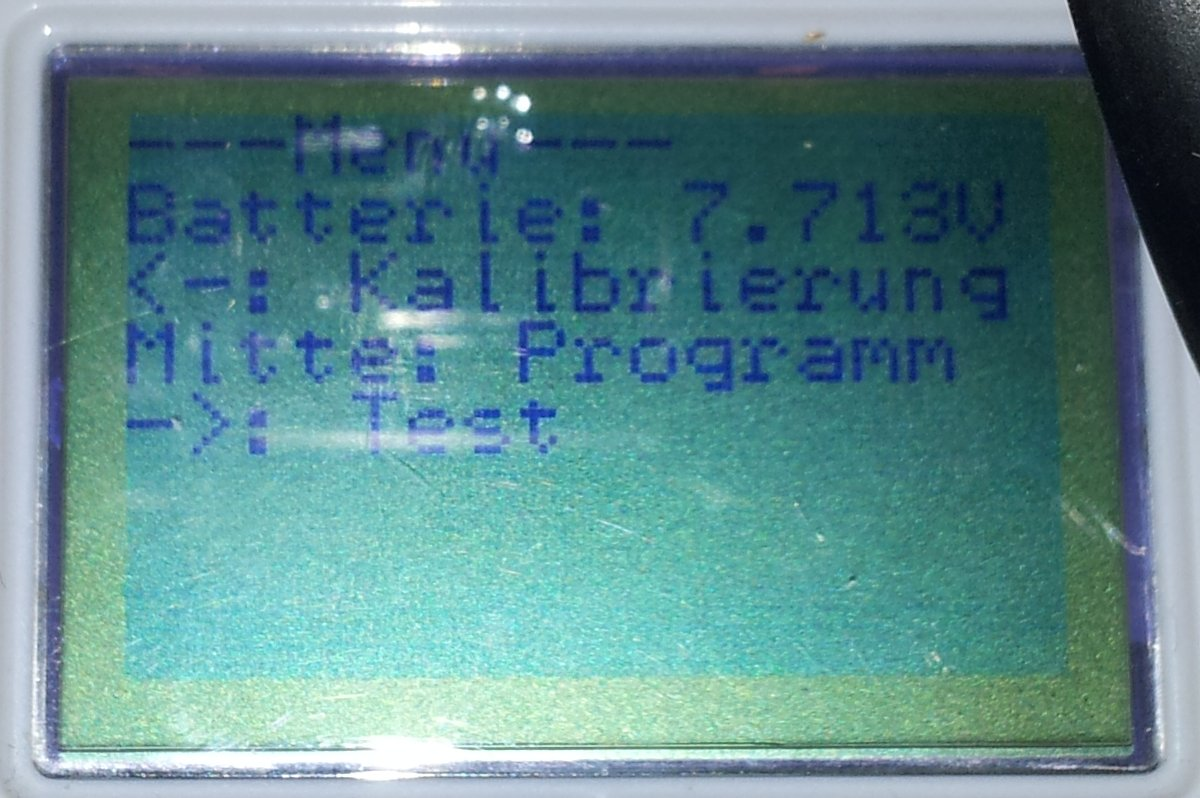
\includegraphics[scale=0.15]{mainscreen.jpg}
\end{figure}

\begin{itemize}
\item Kalibrierung (linker Menüknopf)
\item Programm (mittlerer Menüknopf)
\item Test (rechter Menüknopf)
\end{itemize}

Während der \emph{Kalibrierung} werden halbautomatisch die
Lichtsensoren auf die richtigen Kontrastwerte für die
Linienerkennung konfiguriert. Dabei wird der arithmetische Mittelwert zwischen dem
Untergrund und der Linie ermittelt. Desweiteren werden die Zeiten
gemessen, die für eine Umdrehung auf der Stelle benötigt wird und für
einen fest definierten Kreis. Diese wird später zum Lenken benötigt.

Der Punkt \emph{Programm} enthält die eigentliche Logik. Hier
werden die Hauptroutinen konfiguriert und gestartet, welche den
Roboter autonom fahren lassen.

\emph{Test} beinhaltet verschiedene in sich geschlossene Module um
den Roboter und seine angeschlossenen Sensoren/Motoren zu überprüfen.
Während der Entwicklung wurden in diesem Unterprogramm auch neue
Funktion/Subroutinen isoliert vom Hauptprogramm getestet.

\subsubsection{Das Hauptprogramm}
Das Hauptprogramm unterteilt sich in 2 Tasks: Dem
\emph{Linienfolgealgorithmus} und einer \emph{Kollisionserkennung}.

Der \emph{Linienfolgealgorithmus} läuft die meiste Zeit sichtbar im
Vordergrund und versucht die Strecke abzufahren.

Die \emph{Kollisionserkennung} fragt im Wesentlichen den Status der
beiden Tastsensoren ab. Wird einer der Sensoren gedrückt, wird der
Linienfolgealgorithmus unterbrochen und versucht das vermeintliche
Hindernis zu umfahren. Dafür wäre Multithreading nicht zwingend nötig
gewesen, wenn die Sensoren per Interrupts abfragbar wären.

\subsubsection{Linienfolgealgorithmus}
Der Roboter fährt solange geradeaus, bis er die Linie verliert.
Anschließend sucht der Roboter erst in einem Bereich von 80° auf der
Stelle nach der Linie. Wenn keine Linie vorhanden ist, wird der
Bereich auf 180° ausgeweitet. Der Roboter kann zudem leichte Kurven
erkennen und in diesen mitlenken.

\begin{figure}[ht]
  \centering
  \caption{Suche an der Stelle}
  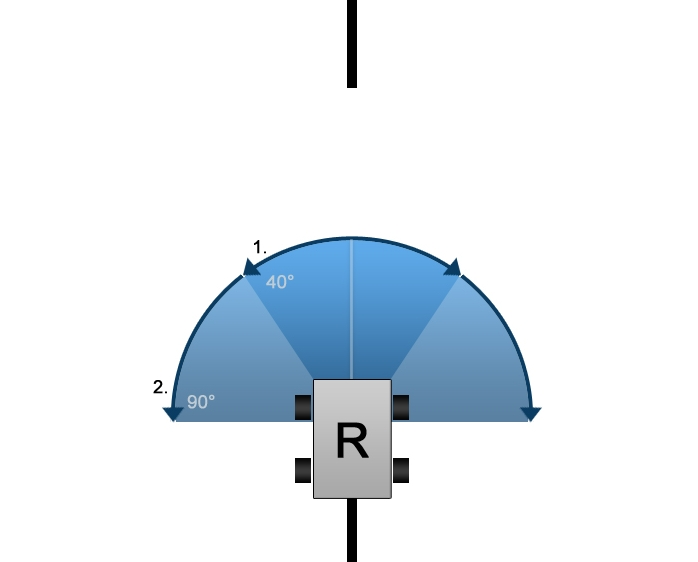
\includegraphics[scale=0.4]{suchnanderstelle.jpg}
\end{figure}

Falls dies keinen Erfolg bringt, sucht der Roboter nach Spitzkehren.
Dazu setzt der Roboter 10cm zurück. Er dreht sich um 40° in beide
Richtungen und fährt jeweils schräg 10cm vorwärts, bis er auf die Linie
trifft.

\begin{figure}[ht]
  \centering
  \caption{Scharfe Kurve}
  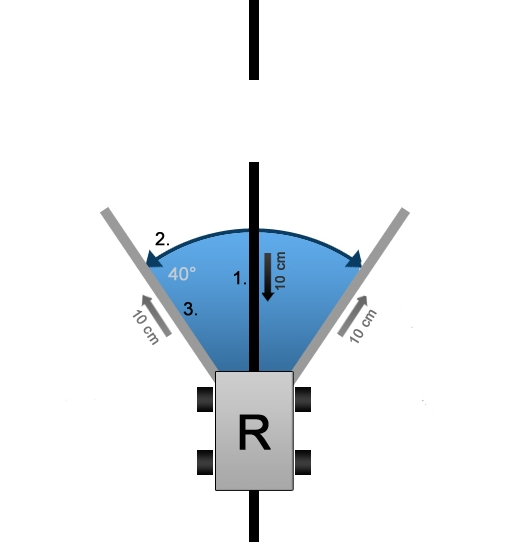
\includegraphics[scale=0.4]{scharfekurve.jpg}
\end{figure}

Wenn keine Linie durch den Roboter erkannt wird, versucht der Roboter
als letztes Mittel einen Kreis zu fahren. Dabei sollen Lücken und
Sackgassen erkannt werden.

\begin{figure}[ht]
  \centering
  \caption{Lücke}
  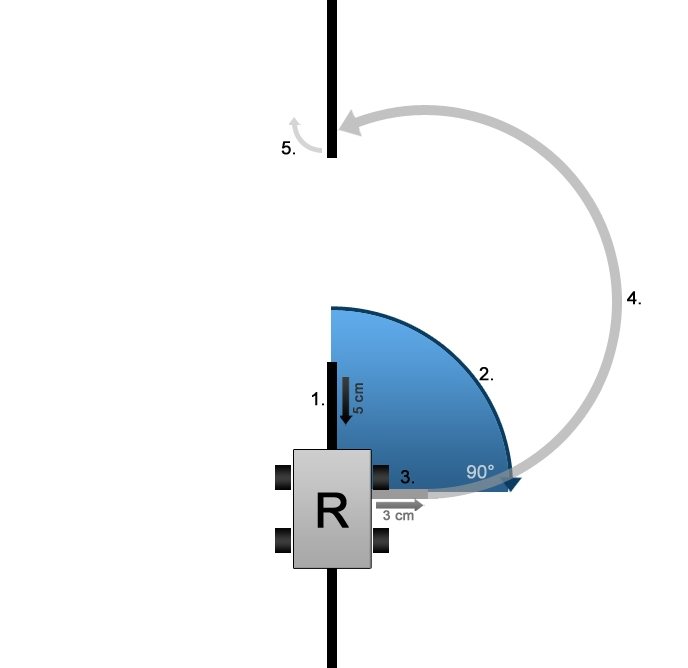
\includegraphics[scale=0.3]{luecke.jpg}
\end{figure}


\subsubsection{Hindernisumfahrung}
Wird einer der Tastsensoren betätigt, versucht der Roboter dieses
Hindernis zu umfahren. Hierfür fährt er ein Stück zurück und dreht danach
um nach links. Danach fährt er vorwärts und schlägt danach einen Kreis nach rechts
ein.

Werden nun die Tastsensoren wieder betätigt, wiederholt sich dieser
Zyklus. Durch dieses Vorgehen tastet er sich um das Hindernis herum, bis
er eine Linie erkennt.

In diesem Fall fährt der Roboter in einer Linkskurve bis er wieder auf
die Linie triff. Auf dieser bringt er sich wieder in Fahrtrichtung und
führt seinen Linienfolgealgorithmus fort.

\begin{figure}[ht]
  \centering
  \caption{Lücke}
  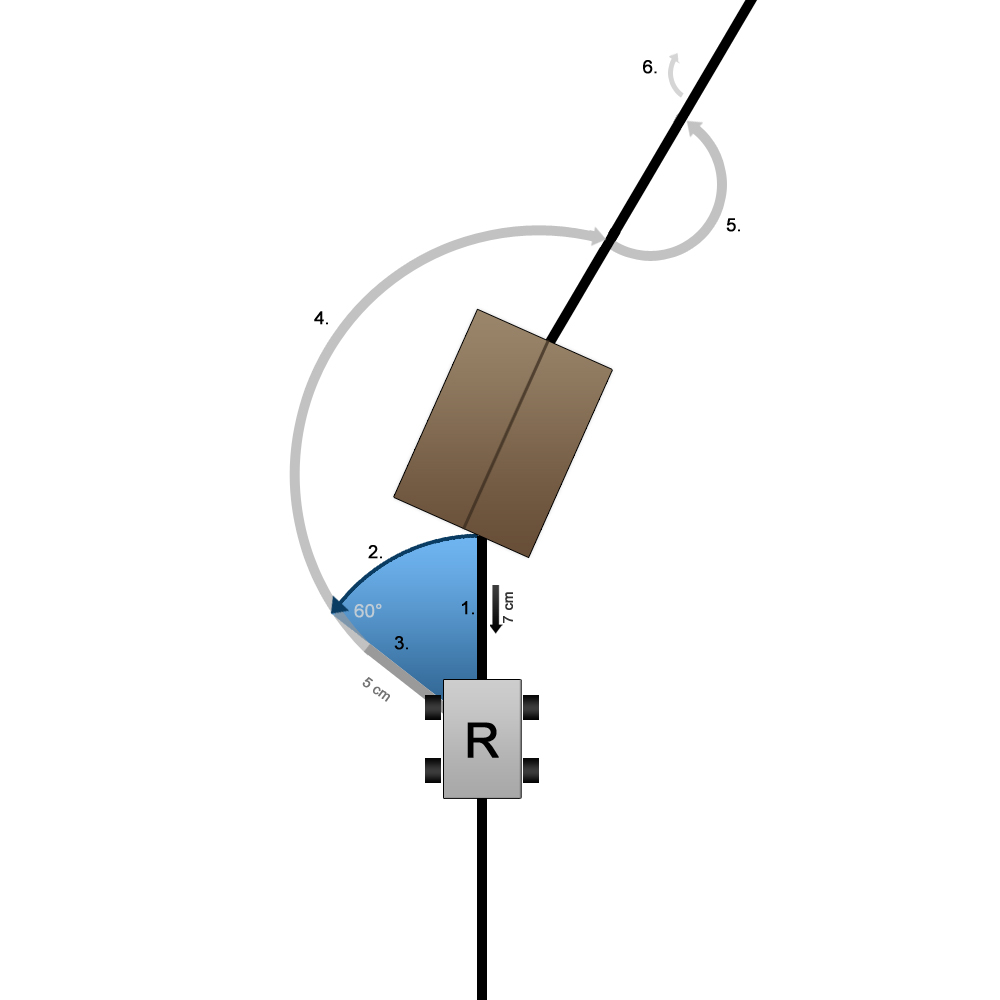
\includegraphics[scale=0.3]{hindernis.jpg}
\end{figure}

\newpage

\subsection{Hardware}

Der Roboter besteht aus:
\begin{itemize}
\item Steuereinheit
\item zwei Servomotoren
\item zwei Tastsensoren
\item Ultraschallsensor
\item Helligkeitssensor
\end{itemize}

Die \emph{Tastsensoren} sind, jeweils links und rechts, am vorderen
Teil des Roboters angebracht. An ihnen ist eine breite, abgerundete
\emph{Stoßstange} befestigt. Diese sorgen dafür, das der Roboter
\emph{Hindernisse} aus allen Winkeln schnell erfassen und somit
umfahren kann.

\begin{figure}[h]
  \centering
  \caption{Tastsensoren mit Stoßstange}
  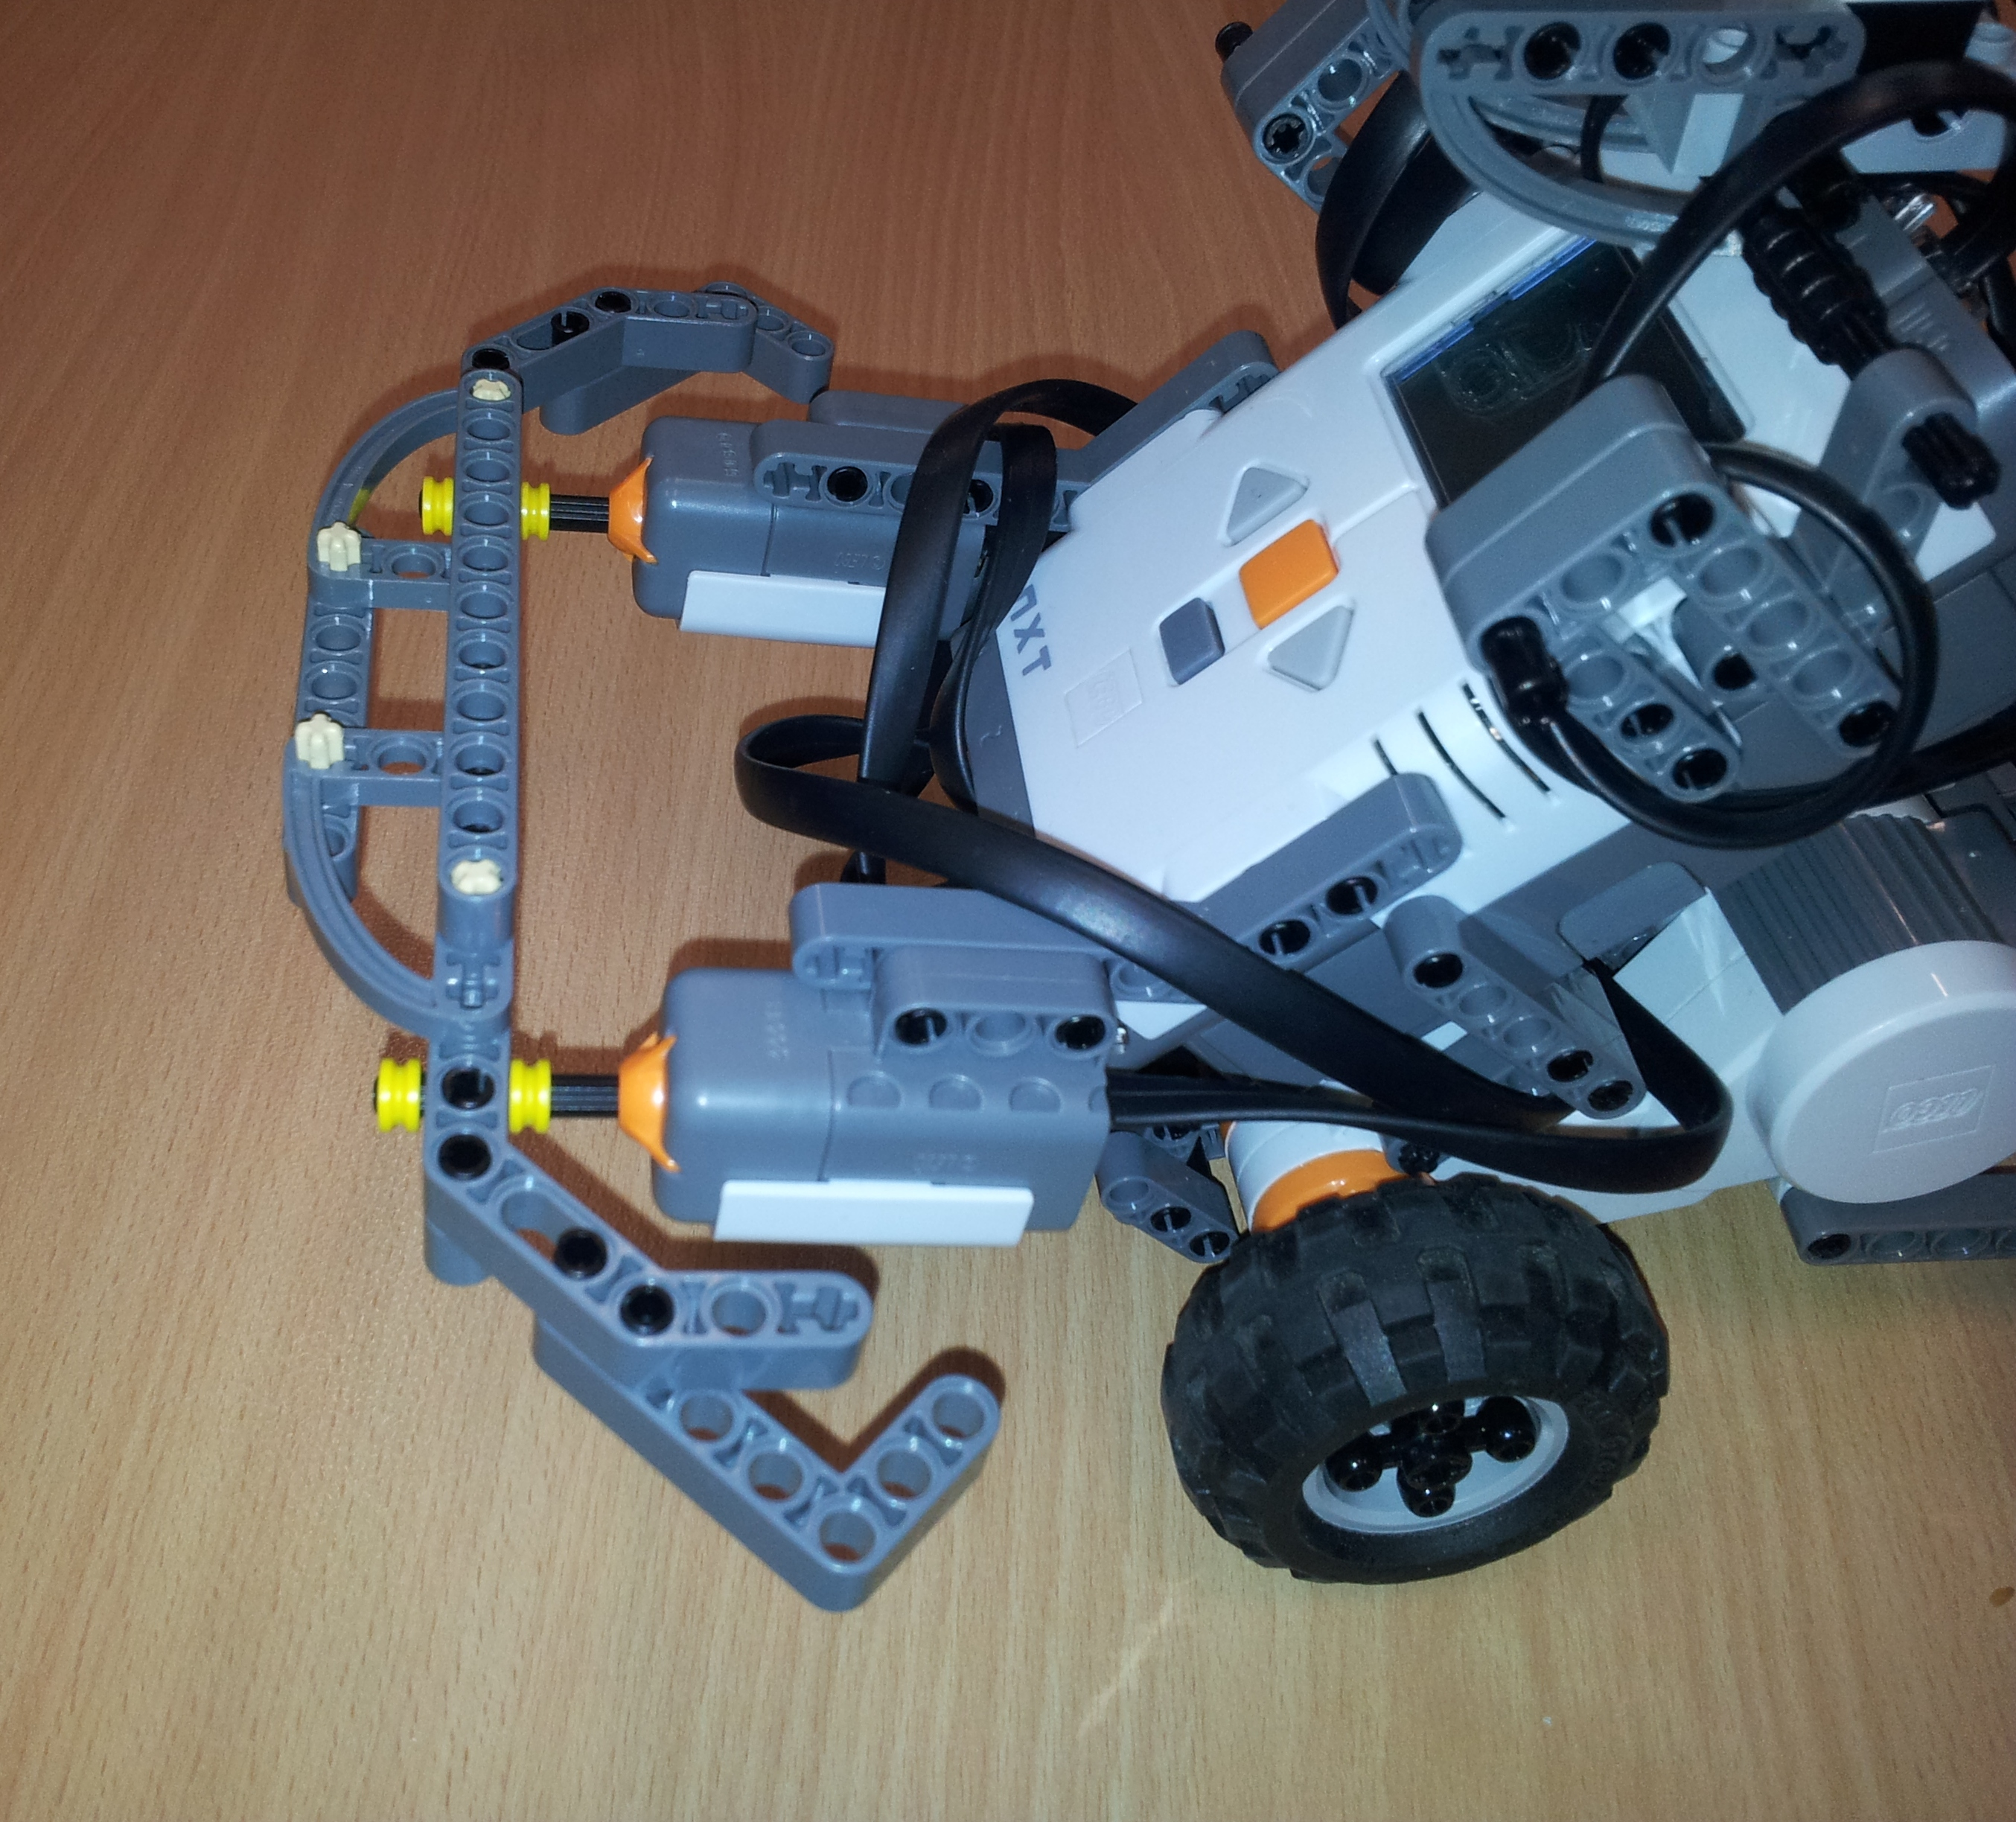
\includegraphics[scale=0.06]{roboter_tastsensor.jpg}
\end{figure}

Der \emph{Lichtsensor} sitzt mittig nah an der \emph{Antriebsachse}.
Er befindet sich zirka einen halben Zentimeter über dem Boden, so dass
etwaige Erschütterungen und Unebenheiten des Roboters keinen Einfluss
auf die Messwerte des Sensors haben. Auf eine zusätzliche Abschirmung
wurde verzichtet, da der Sensor im Raw-Modus schon gute Kontrastwerte
liefert.

\begin{figure}[h]
  \centering
  \caption{Lichtsensor}
  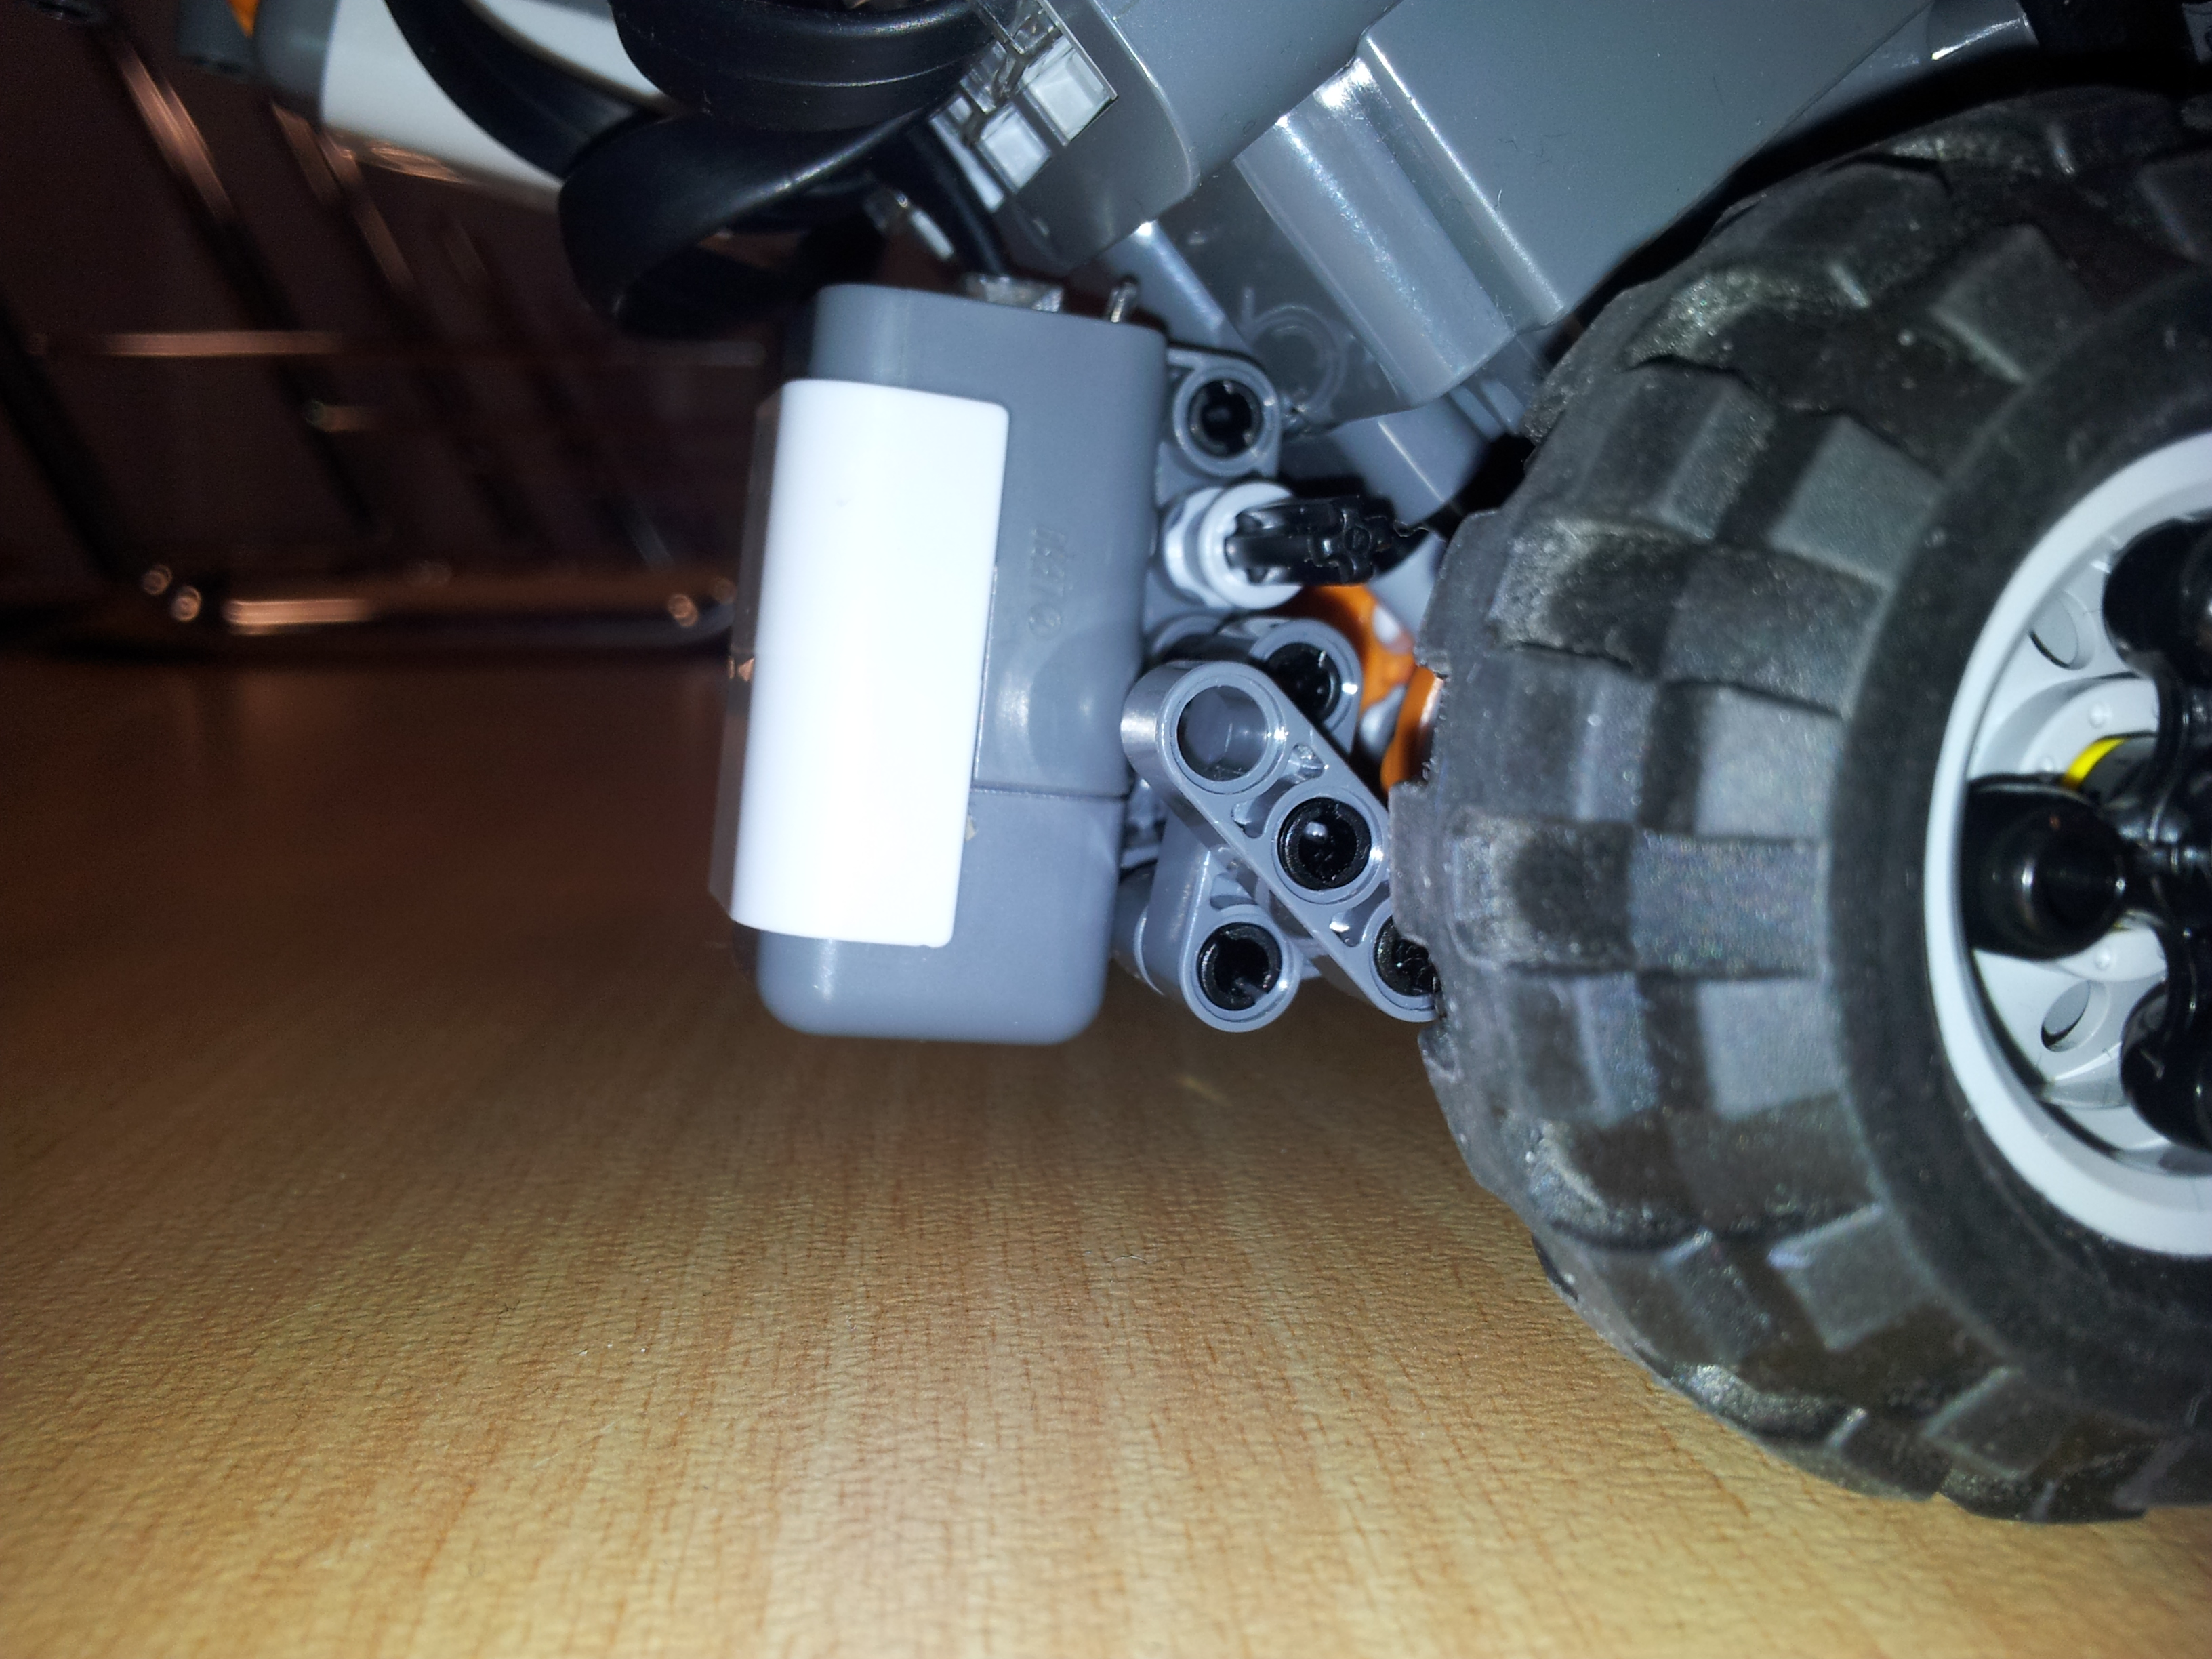
\includegraphics[scale=0.06]{roboter_lichtsensor.jpg}
\end{figure}

Die \emph{Antriebsachse} mit den zwei Motoren befindet sich unten
mittig am Roboter. Damit der Roboter sowohl stabil als auch wendig
ist, wurde hinten mittig eine \emph{Kugelhalterung} angebaut. Die
eingefasste Kugel ist starr und dreht sich beim Fahren nicht. Diese
Kugel hat gegenüber eines Stützrades den Vorteil, dass diese wendiger
ist und sich in jeder Situation gleich verhält.

\begin{figure}[h]
  \centering
  \caption{Antriebsachse}
  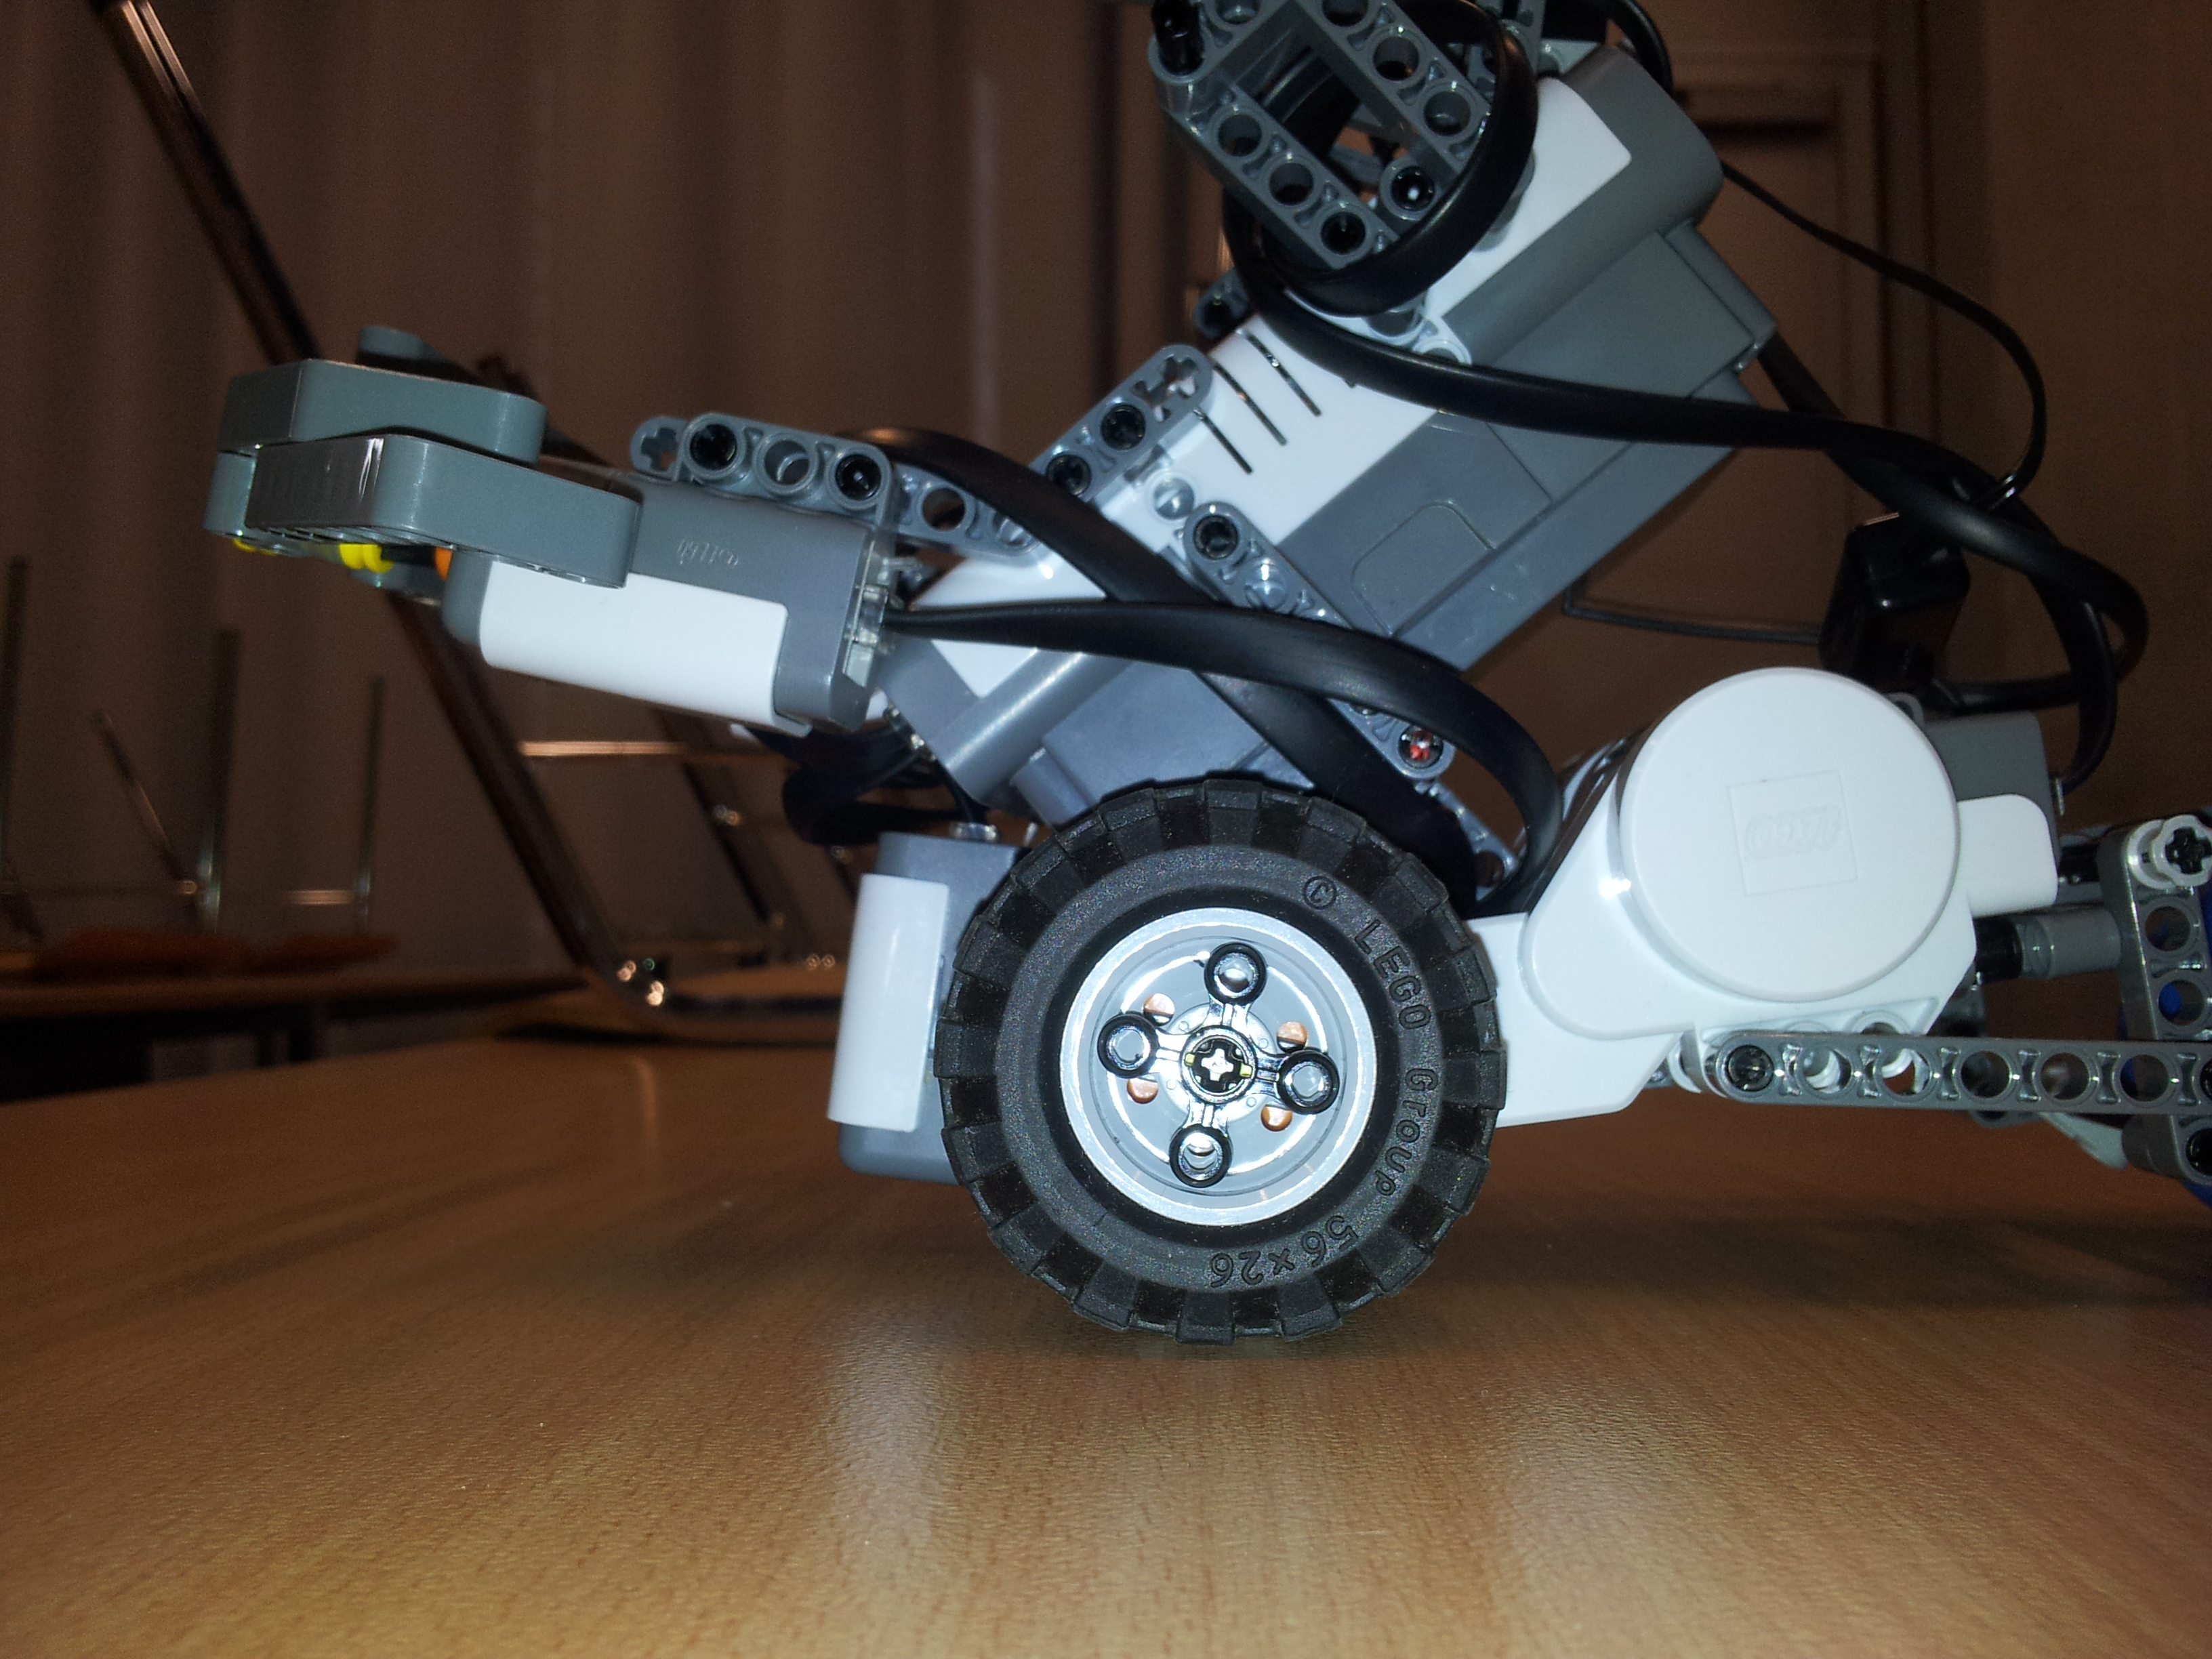
\includegraphics[scale=0.06]{roboter_antriebsachse.jpg}
\end{figure}

\newpage

Der \emph{Ultraschallsensor} sitzt mittig auf dem Roboter. Eine
Funktion für diesen war geplant, wurde aber während der Entwicklung
verworfen. Er dient also nur als Ergänzung des optischen Erscheinungsbildes.

\begin{figure}[h]
  \centering
  \caption{Ultraschallsensor}
  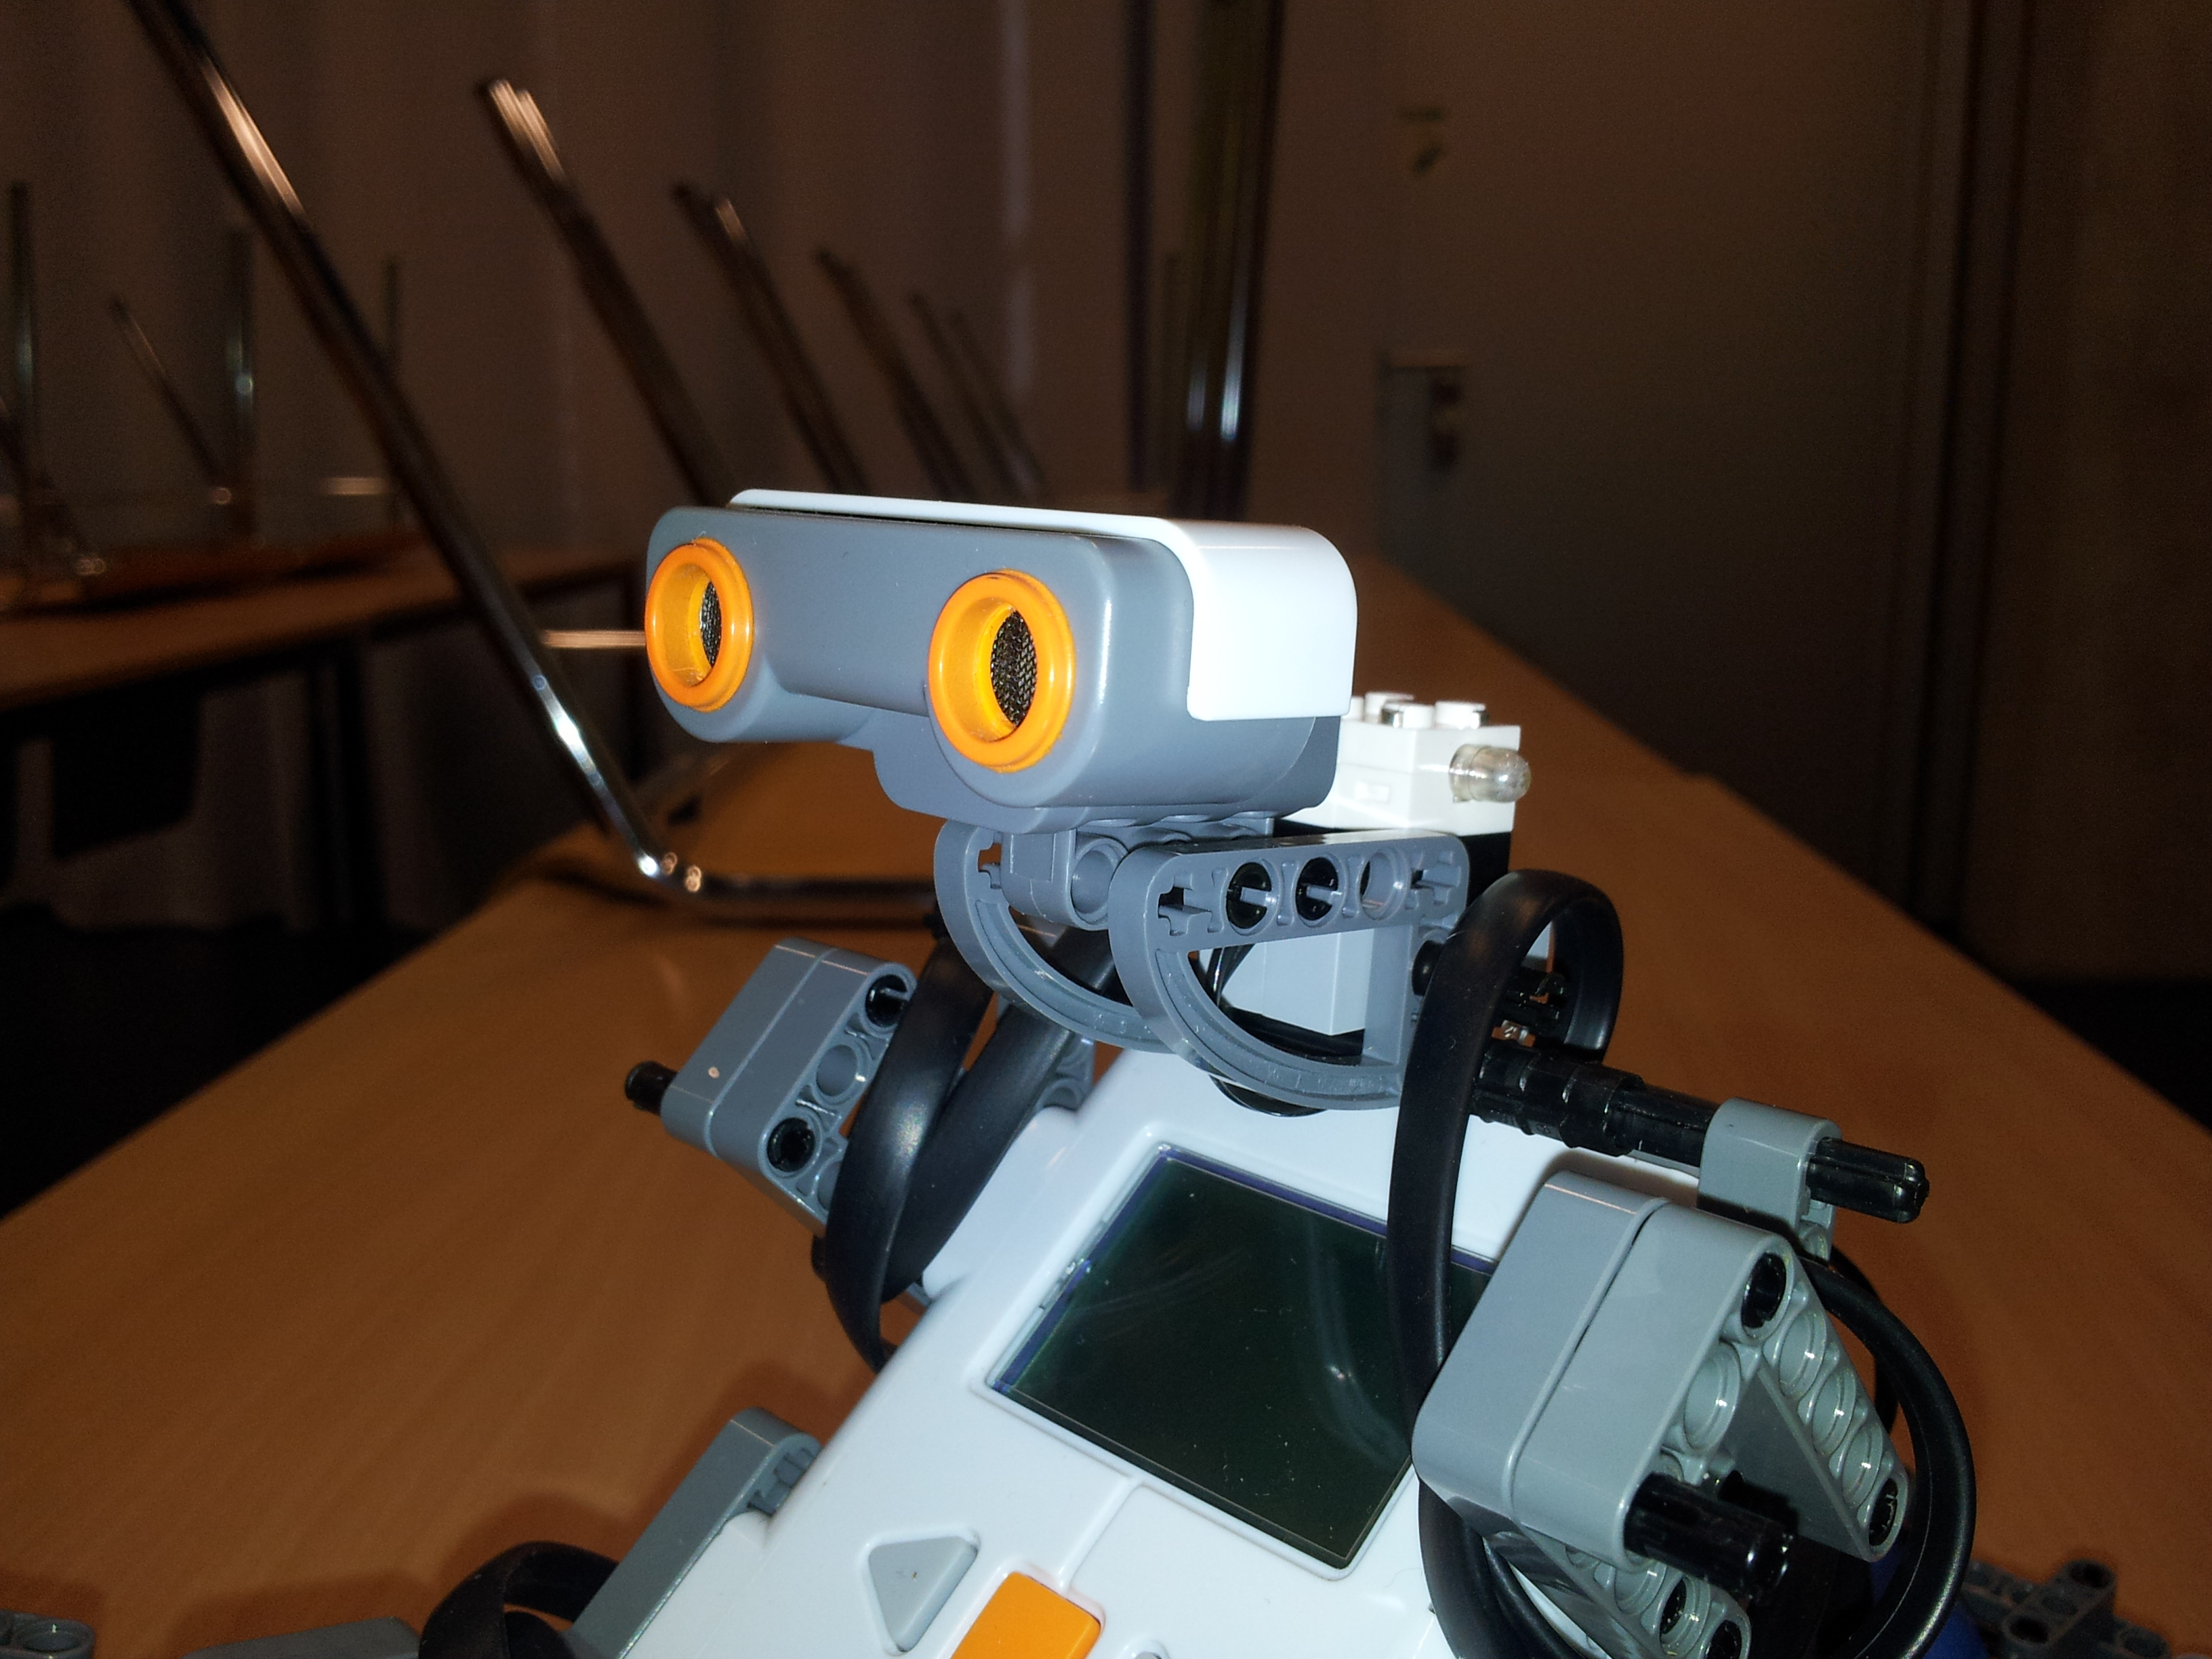
\includegraphics[scale=0.06]{roboter_ultraschallsensor.jpg}
\end{figure}

Die \emph{Steuereinheit} sitzt zentral auf dem Roboter, sodass der
Roboter einerseits optimal ausbalanciert ist und andererseits die
Tasten der \emph{Steuereinheit} gut zugänglich sind.

\begin{figure}[h]
  \centering
  \caption{Steuereinheit}
  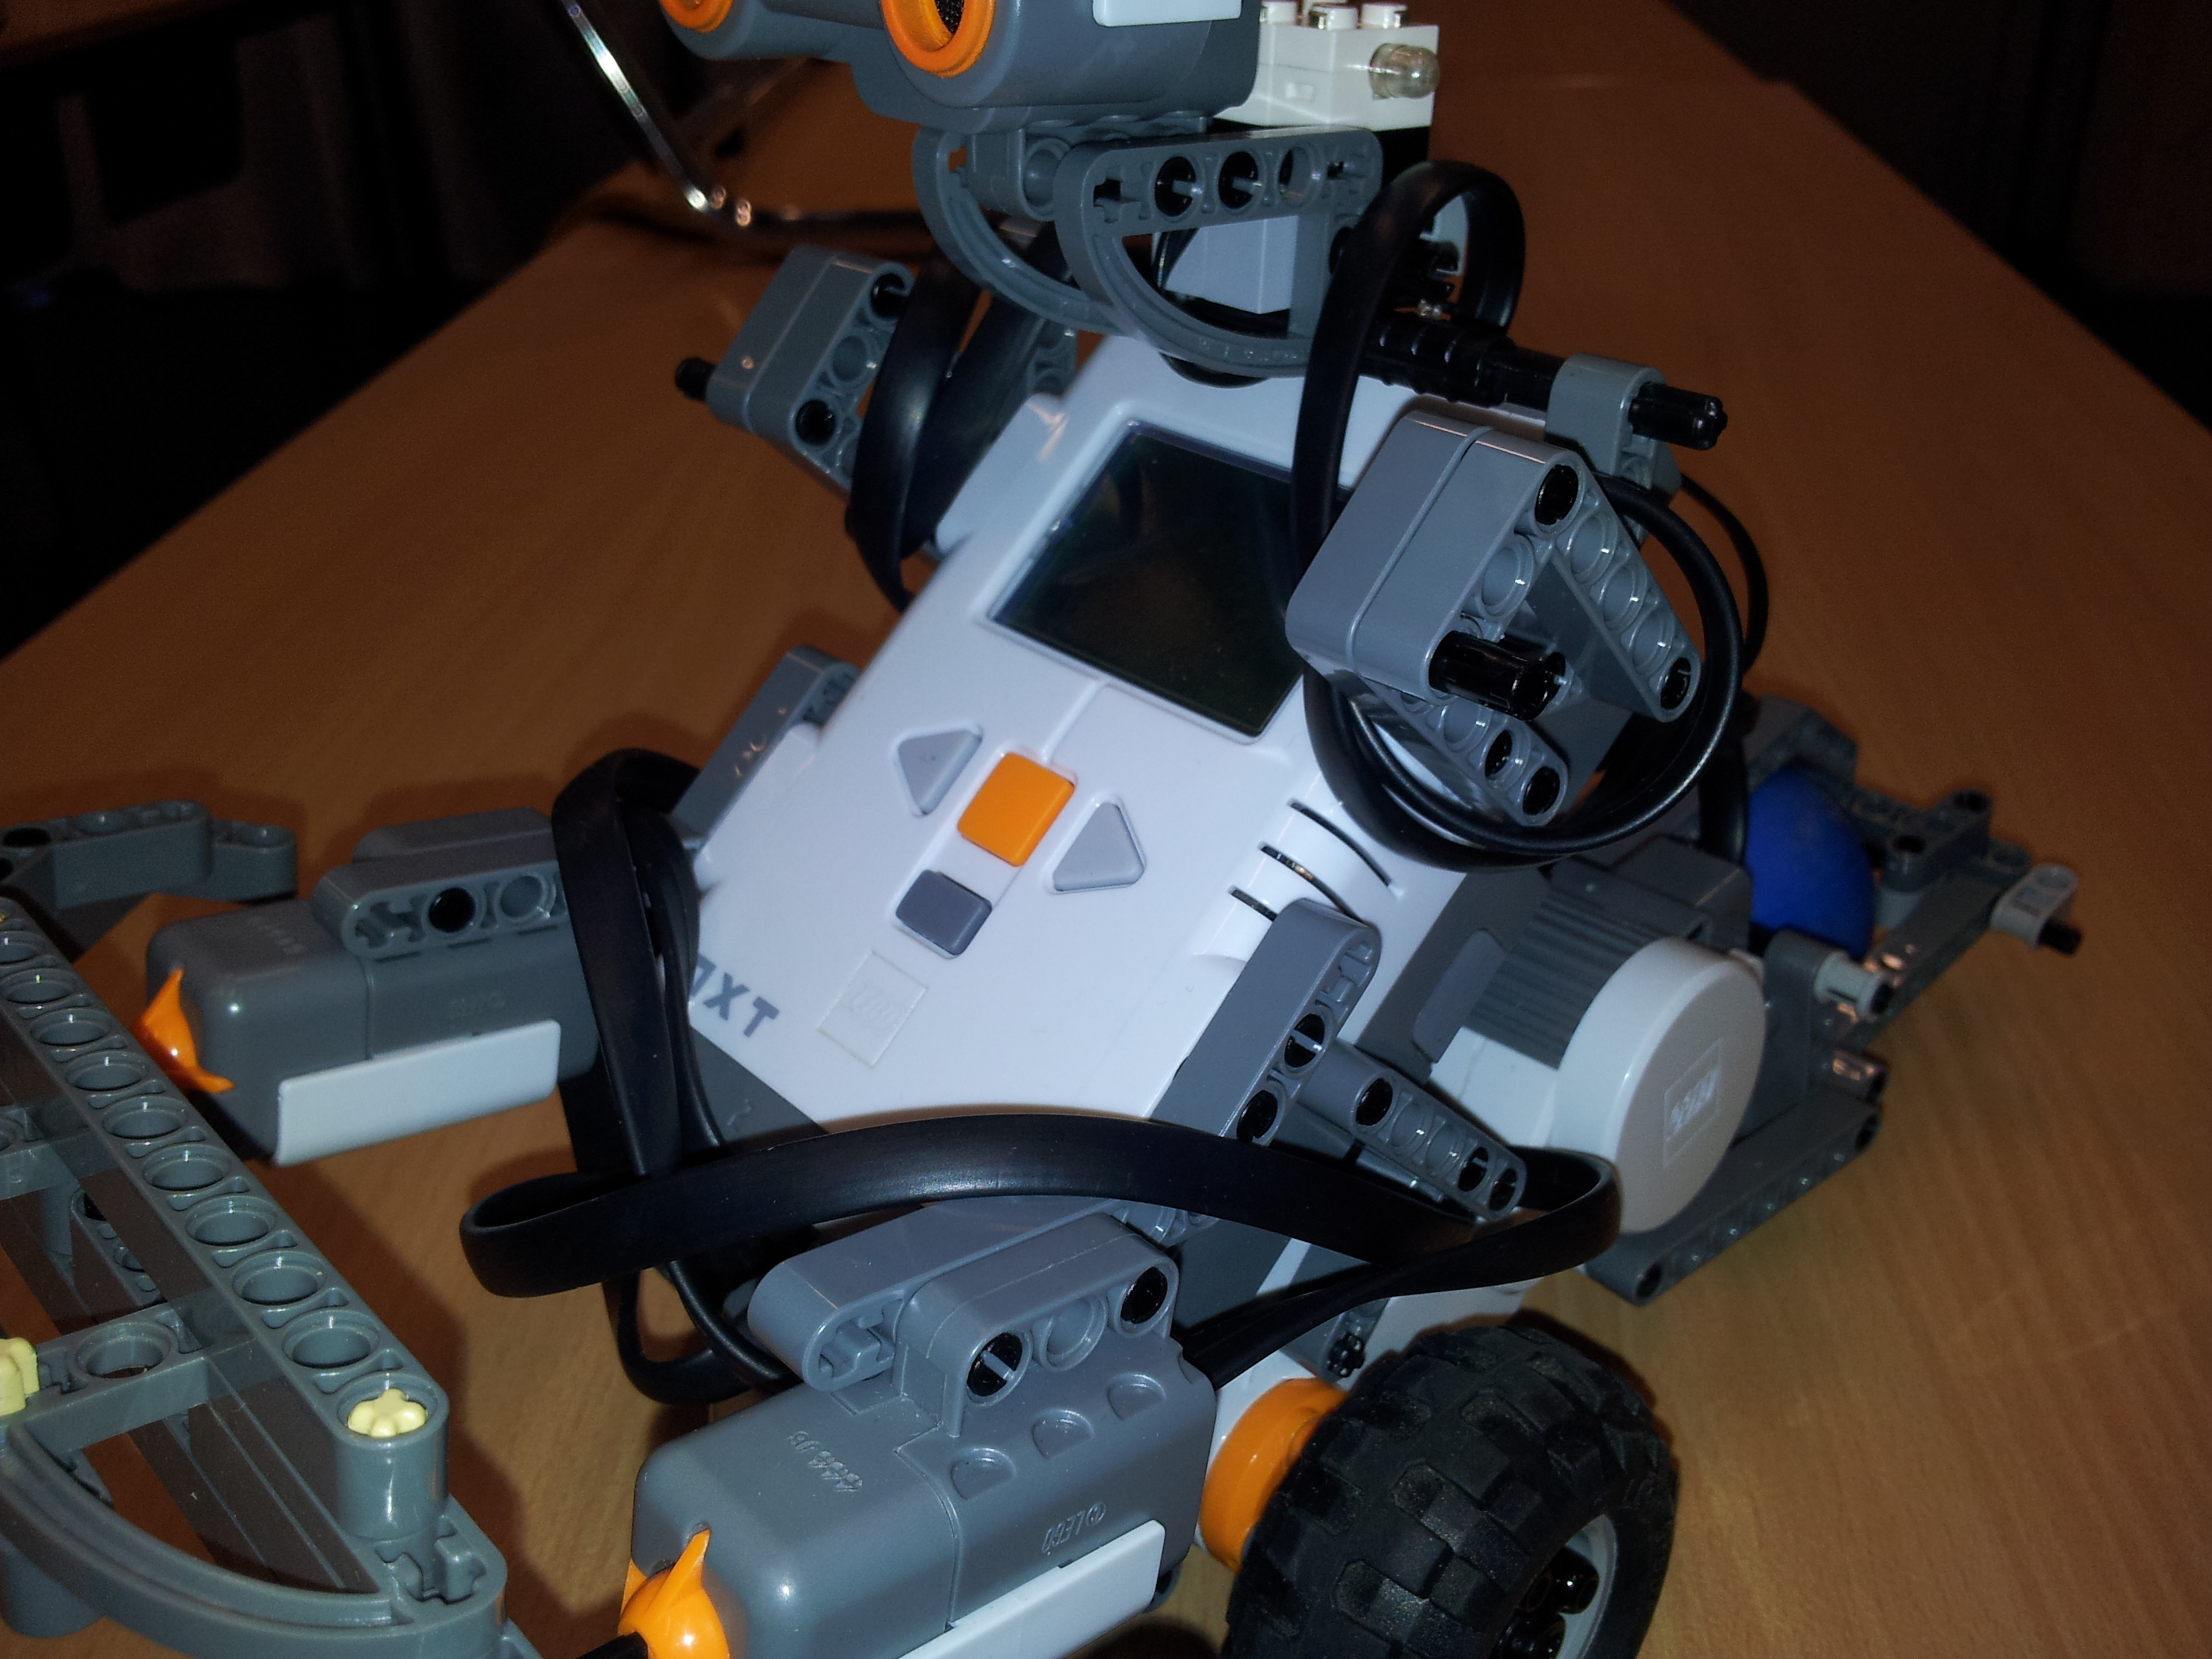
\includegraphics[scale=0.06]{roboter_steuereinheit.jpg}
\end{figure}

\newpage

Insgesamt ist der Roboter 30 cm lang, 21 cm breit und 19 cm hoch.

\begin{figure}[h]
  \centering
  \caption{gesamter Roboter}
  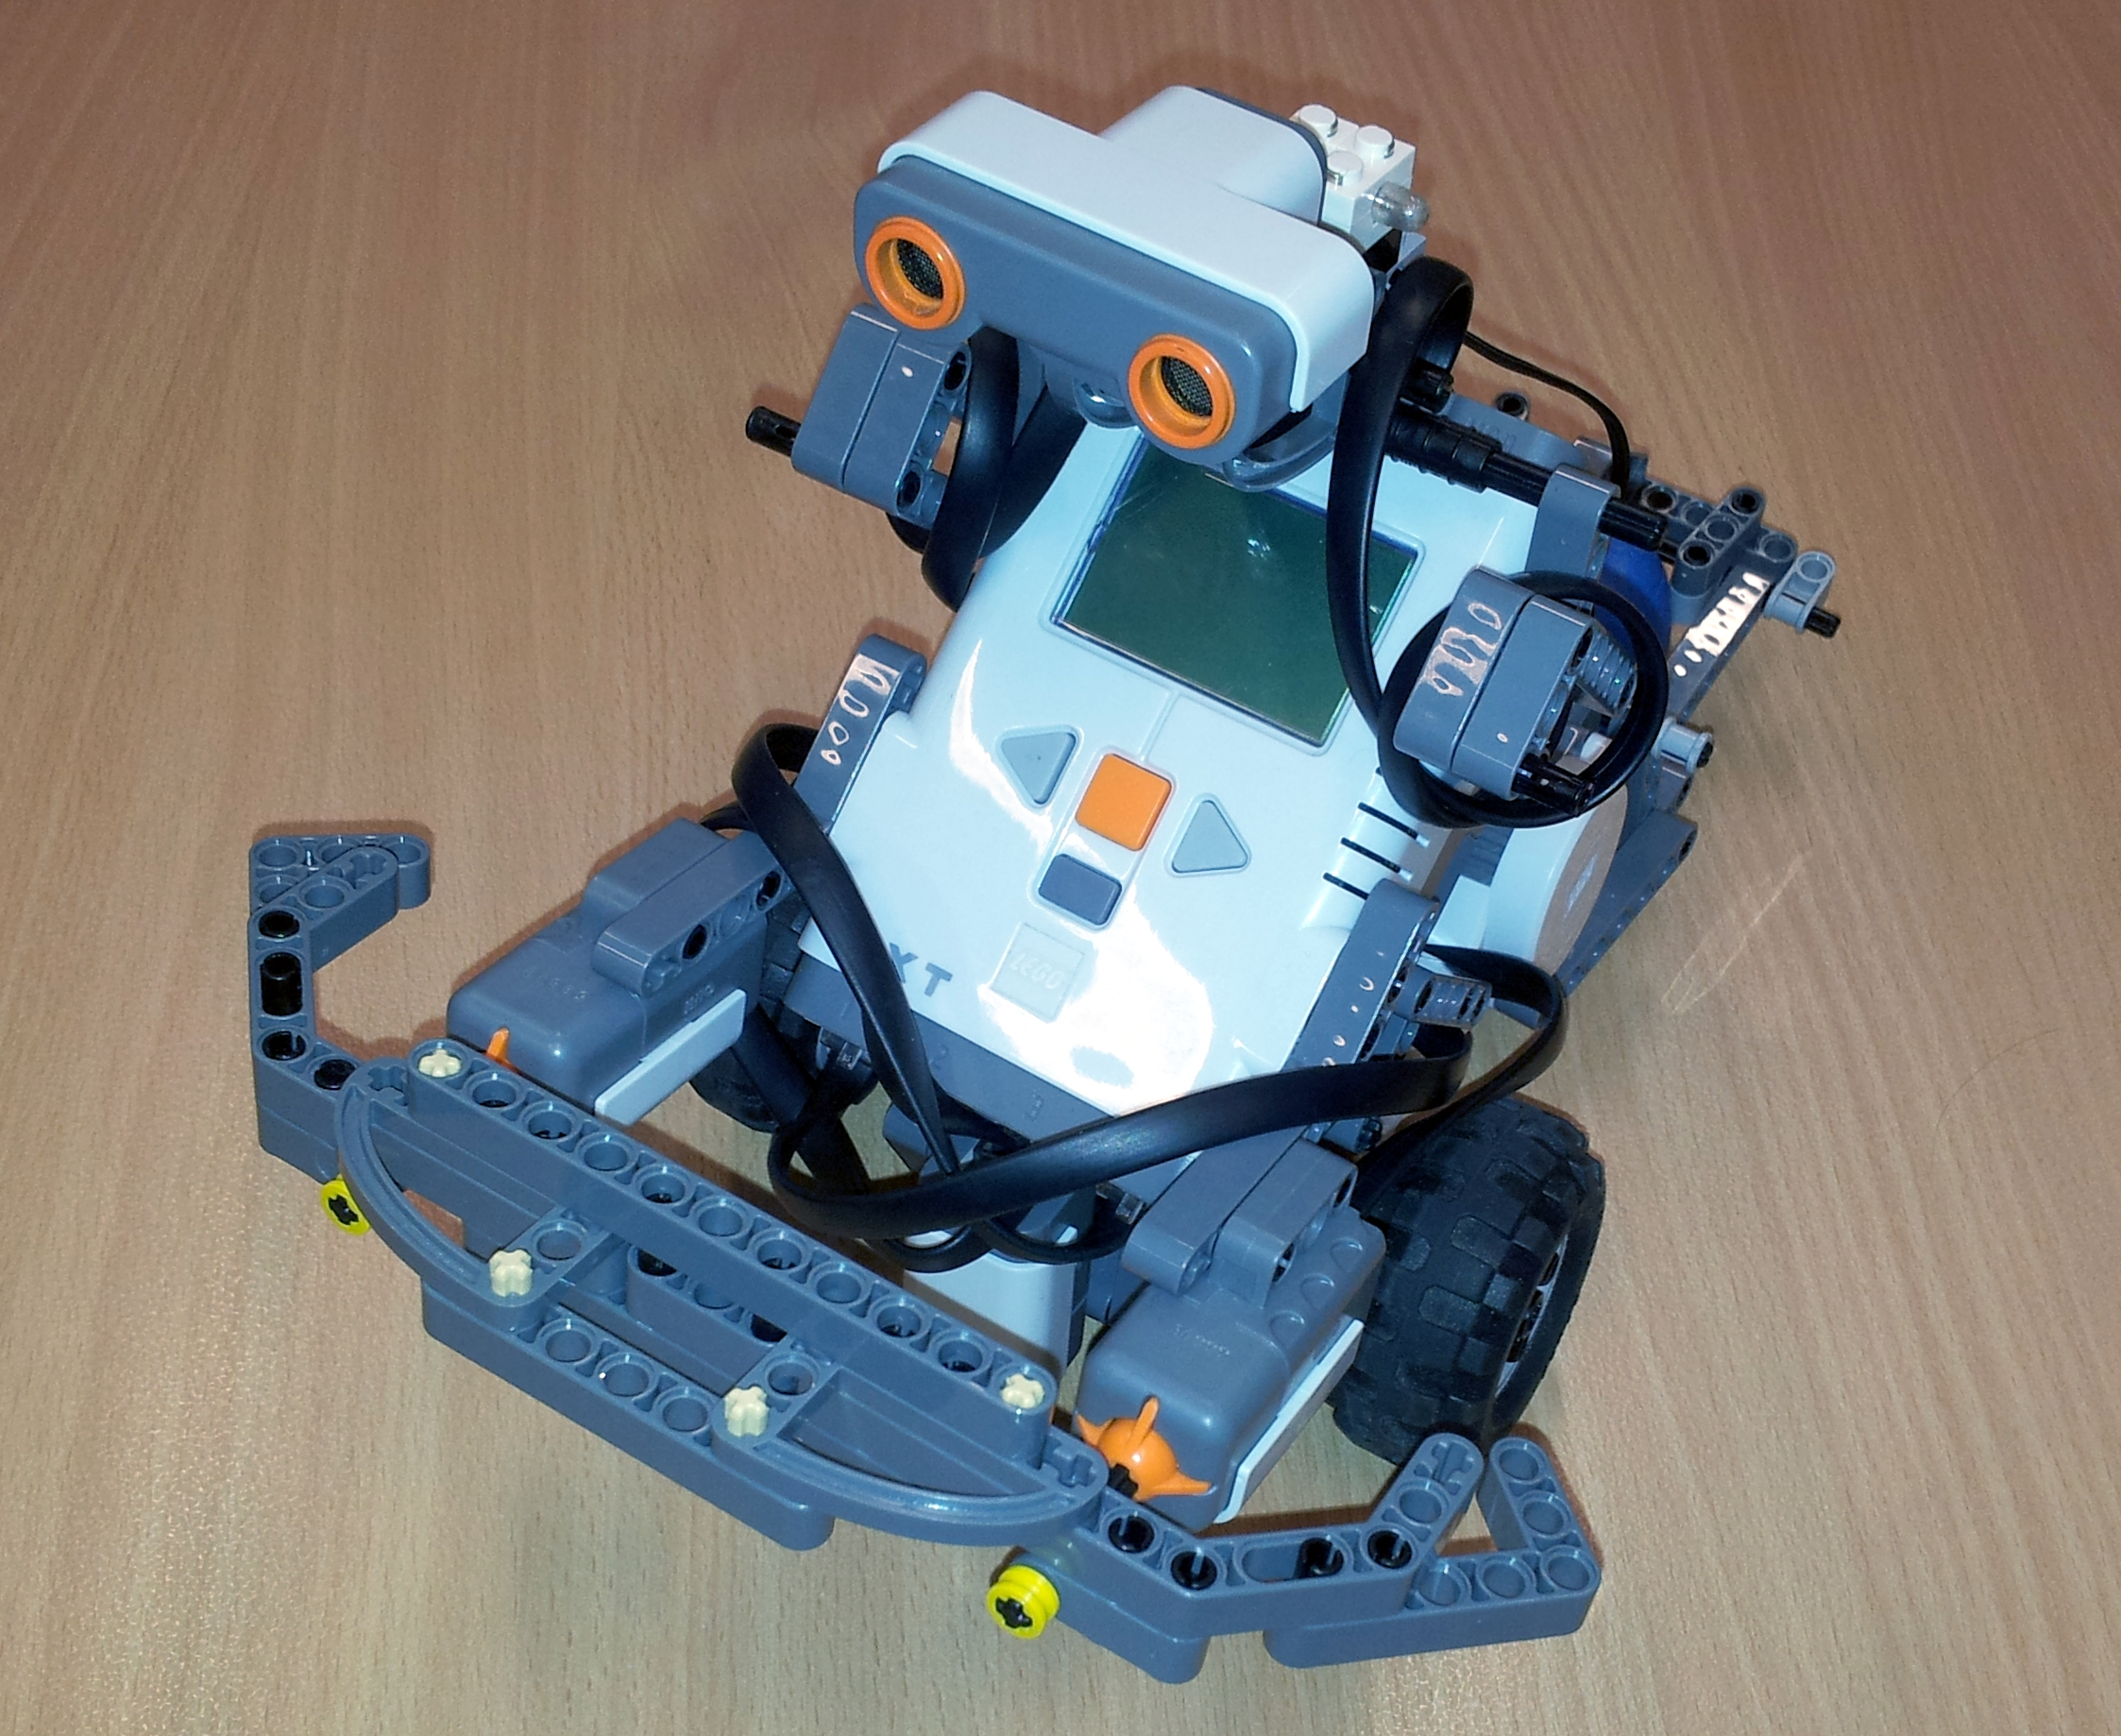
\includegraphics[scale=0.15]{roboter_gesamt.jpg}
\end{figure}

\section{Projektverlauf und Erfahrungen}
\subsection{Lösung der Aufgabe}

Als erstes haben wir die grundlegenden Aufgaben, welche an den Roboter
gestellt wurden, \emph{zusammengefasst}. Wir analysierten die Videos
des ersten Kurs-Durchganges. Dadurch bekamen wir einen guten Einblick,
mit welchen Problemen die Roboter zu kämpfen haben und welche
Lösungsansätze/Bauweisen sich bewährten.

Nebenbei baute ein Teil der Gruppe aus den gegebenen Teilen des
Bausatzes den Roboter, wobei \emph{eigene Ideen} im gleichen Maße
Einfluss fanden wie vorgegebene Bauanleitungen aus dem Bausatz oder
dem Internet. Es wurden Funktionen für grundlegende Bewegungsformen
wie Kurven, Kreisfahrt oder das Fahren einer bestimmten Länge
programmiert.

Im Anschluss arbeiteten wir Schritt für Schritt die zu erfüllenden
Aufgaben in das Programm ein, wobei \emph{grundlegende Aufgaben} wie
dem \emph{folgen einer Linie} Vorrang vor Aufgaben wie der
\emph{Bewältigung von Lücken} oder \emph{Spitzkehren} hatten. Parallel
hierzu testen wir permanent die eingearbeiteten Funktionen auf
diversen Teststrecken, um etwaige Fehler im Programmcode schnell zu
erkennen und zu beheben.

Dieser Teil war mit Abstand der zeitaufwendigste Teil unserer Arbeit,
da erst hier auch kleine Fehler im Programm sichtbar wurden, welche
erst beim intensiven Testen offensichtlich wurden.

Nach Fertigstellung des Roboters wurde dieser nochmals permanent
getestet, um sicherzugehen, dass dieser \emph{zuverlässig} und
\emph{fehlerfrei} die vorgegebenen Strecken absolvieren kann. Hierbei
wurden nochmals auftretende Fehler ausgebessert.

\subsection{Welche eurer Entscheidungen waren gut und welche nicht?}

Es hat sich als positiv herausgestellt, dass wir den Roboter nicht
stur nach einer vorgegebenen Bauanleitung bauten, sondern auch eigene
Ideen mit einfließen liesen. Hierdurch konnten wir den Roboter vom
Design her ganz nach unserem Geschmack bauen. Darüber hinaus war es
ein großer Vorteil, dass wir permanent während der Entwicklung der
Software nicht nur diese an den Roboter anpassen konnten, sondern auch
auftretende funktionelle Probleme durch bauliche Änderungen behoben
werden konnten.

Eine negative Entscheidung war, dass wir unsere Änderungen bei der
Behebung von Fehlern nicht dokumentierten, da somit nicht
nachvollziehbar war, wodurch eventuell neu auftretende Fehler
verursacht wurden. In diesem Fall mussten wir im Ernstfall komplexe
Änderungen verwerfen und Teile des Programms überarbeiten, um den
ursprünglich kleinen Fehler zu beheben.

\subsection{Eigene Erkenntnisse}

Mit unserem jetzigen Kenntnisstand würden wir uns vor dem Projekt
einen \emph{Arbeitsplan} aufstellen, in welchem die Verteilung der
anstehenden Aufgaben auf die \emph{einzelnen Gruppenmitglieder}
festgelegt ist. Dies hätte dann den Vorteil, dass man anstatt
gemeinsam alle Aufgaben zu bewältigen sich jeder Einzelne auf
bestimmte Aufgaben \emph{spezialisieren} kann und somit im Endeffekt
\emph{besser} und \emph{effizienter} gearbeitet werden kann.

\subsection{Implementierung und Verbesserung}
Zum einen wäre es möglich, die Lösung einzelner spezieller Aufgaben
\emph{effizienter} zu gestalten, insbesondere die der
\emph{Hindernisumfahrung}. Es besteht hierbei die Möglichkeit, neben
den \emph{Tastsensoren} auch den \emph{Ultraschallsensor} mit
einzubeziehen, da man durch diesen die Hindernisse nicht immer
anstoßen muss, um sie zu erfassen, sondern diese bereits in einer
gewissen Distanz erfasst und umfahren werden können. Hierdurch würde
man die zu fahrende Strecke und auch Zeit minimieren, welche
der Roboter zur Hindernisumfahrung benötigt. Ein Ultraschallsensor
könnte zudem Spezialfälle wie Hindernisse, welche als Sackgassen
aufgebaut sind, abdecken.

Zum anderen könnte man die \emph{Kugelhalterung} verbessern, da diese
in ihrer jetzigen Fassung die Kugel einklemmt und diese somit nicht
rollen kann, sondern schleift. Eine ideale Kugelhalterung würde
einerseits gewährleisten, dass die Kugel nicht aus ihr
\emph{herausspringt}, und andererseits dass diese rollen kann und
nicht schleift.

Eine weitere Verbesserungsmöglichkeit wäre, die Position der
\emph{Steuereinheit} zu verändern, da in ihrer jetzigen Position der
\emph{Ladekabelanschluss} verdeckt ist und somit beim Laden des
Roboters ein \emph{Auseinanderbauen} unumgänglich ist.

\section{Bewertung}
\subsection{Einschätzung und Nutzen des Projektes}

Das Projekt war eine gute Gelegenheit, unsere ersten
\emph{Programmierkentnisse} praktisch anzuwenden. Es war insbesondere
sehr befriedigend, dass man die Auswirkung einer jeden Änderung im
Programm sofort am Roboter sah, und somit ein direktes \emph{Feedback}
der eigenen \emph{Erfolge} und \emph{Misserfolge} bekam. Dadurch
erhöhte sich auch der \emph{Spaßfaktor}, weil ein stetiger Erfolg gut
für die eigene Motivation war.

Darüberhinaus war es auch eine gute Gelegenheit, das gemeinsame
Arbeiten an einem Projekt zu erlernen und dabei im Umgang mit
Versionswaltungen wie \emph{Git} sicherer und vertrauter zu werden.

Weiterhin wurde man beim Anfertigen des Abschlussberichtes vertrauter
im Umgang mit \LaTeX. Dies ist von Vorteil, da Latex im
\emph{universitären Umfeld} sehr verbreitet ist und sich gut für
Dokumentationen/Abschlussarbeiten eignet.

\subsection{Verbesserungsvorschläge}

Da den Meisten der Umgang mit \emph{NXC}, \LaTeX und \emph{Git} nicht
vertraut war, und es zudem keine Einführung in diesem Sinne gab, wurde
man mehr oder weniger "`ins kalte Wasser geschmissen"'. Den Umgang mit
diesen Programmen und Programmiersprachen mussten wir uns selber
aneignen, wodurch ein Teil der zur Verfügung stehenden Zeit verloren
ging. Somit wäre eine kurzer \emph{Crashkurs} zum Beispiel im Rahmen
eines \emph{Workshop} wünschenswert. Diese könnte in Form von
einzelnen Gruppen durch die jeweiligen \emph{Tutoren} am Anfang des
Kurses stattfinden. Da hier gegenüber Vorlesungen der Vorteil besteht,
dass \emph{Unklarheiten} und \emph{Fragen} sofort diskutiert werden
können.

\end{document}
